\chapter{Concepts de base}
\label{chap:concept}

\section{Introduction}

Ce chapitre pose le vocabulaire utilisé dans la suite du mémoire. Quatre notions reviennent sans cesse : l'essaim, le voisinage, le graphe sur lequel circulent les informations, et la manière dont la qualité d'une formation se mesure. Elles sont décrites ici à un niveau général. Les choix concrets, c'est-à-dire les valeurs de paramètres, les équations et les conventions de mesure, viennent dans les chapitres suivants. La seule figure du chapitre provient d'un épisode réel, mais elle sert à illustrer une notion, pas à juger un résultat.

Une précaution d'abord. Décrire un mécanisme ne montre pas qu'il fonctionne. Dire qu'un réseau à passage de messages accepte un nombre variable de voisins décrit une propriété de calcul, pas un résultat. Cette distinction, entre ce que le code rend possible et ce qu'une campagne mesure, traverse tout le mémoire.

\section{Essaim, localité, décentralisation}

En robotique en essaim, le comportement collectif naît de décisions prises localement par des robots assez simples, qui échangent peu d'information \cite{brambilla2013}. L'idée s'oppose à un pilotage unique qui connaîtrait tout du groupe. Les tâches sont réparties, ce qui rend le groupe moins sensible à la panne d'une unité et plus facile à agrandir. En contrepartie, la coordination est plus difficile à obtenir.

Trois notions sont à distinguer. Un contrôleur \emph{centralisé} lit toutes les positions et calcule toutes les commandes. Un contrôleur \emph{décentralisé} ne laisse à chaque robot que ses informations et celles de ses voisins. L'\emph{apprentissage}, lui, peut rester global : rien n'empêche d'ajuster des poids à partir d'une mesure calculée sur l'essaim entier, tant que l'exécution ne dépend plus que d'observations locales. C'est le schéma retenu ici. La décentralisation porte donc sur la décision de mouvement, pas sur l'entraînement.

Cette précision évite une confusion classique. Une politique exécutée localement peut avoir été entraînée avec une information qu'aucun robot ne possède pendant l'exécution. Elle n'en devient pas centralisée, mais sa qualité dépend de l'écart entre les deux situations. Une comparaison entre contrôleurs ne vaut donc que si les deux reçoivent la même information. C'est une exigence méthodologique, pas un fait acquis. Au chapitre~\ref{chap:experiences}, la règle manuelle reçoit d'ailleurs un peu plus d'information que le GNN, et nous en tenons compte dans la lecture des résultats.

\section{Voisins, portée de communication et graphe de proximité}

Dans un essaim, ce qu'un robot sait dépend de ce qu'il perçoit et de ce que ses voisins lui transmettent. Le voisinage n'est pas une liste fixe : il change à chaque pas, au fil des déplacements. On le définit d'habitude par une portée : deux robots échangent si leur distance ne dépasse pas une valeur fixée. L'ensemble de ces liens forme un graphe, dont les nœuds sont les robots et les arêtes les communications possibles. Ce graphe est recalculé à chaque pas. Un robot peut donc passer d'isolé à très connecté sans que le programme change.

La Figure~\ref{fig:communication-graph} montre ce graphe sur un épisode réel, au départ et à la fin. Le robot marqué d'une étoile échange avec tous les robots situés dans le cercle pointillé, et avec eux seulement. Au départ, il a 22 voisins sur 39. À la fin, quand l'essaim s'est resserré sur la figure, il en a 26.

\begin{figure}[htbp]
  \centering
  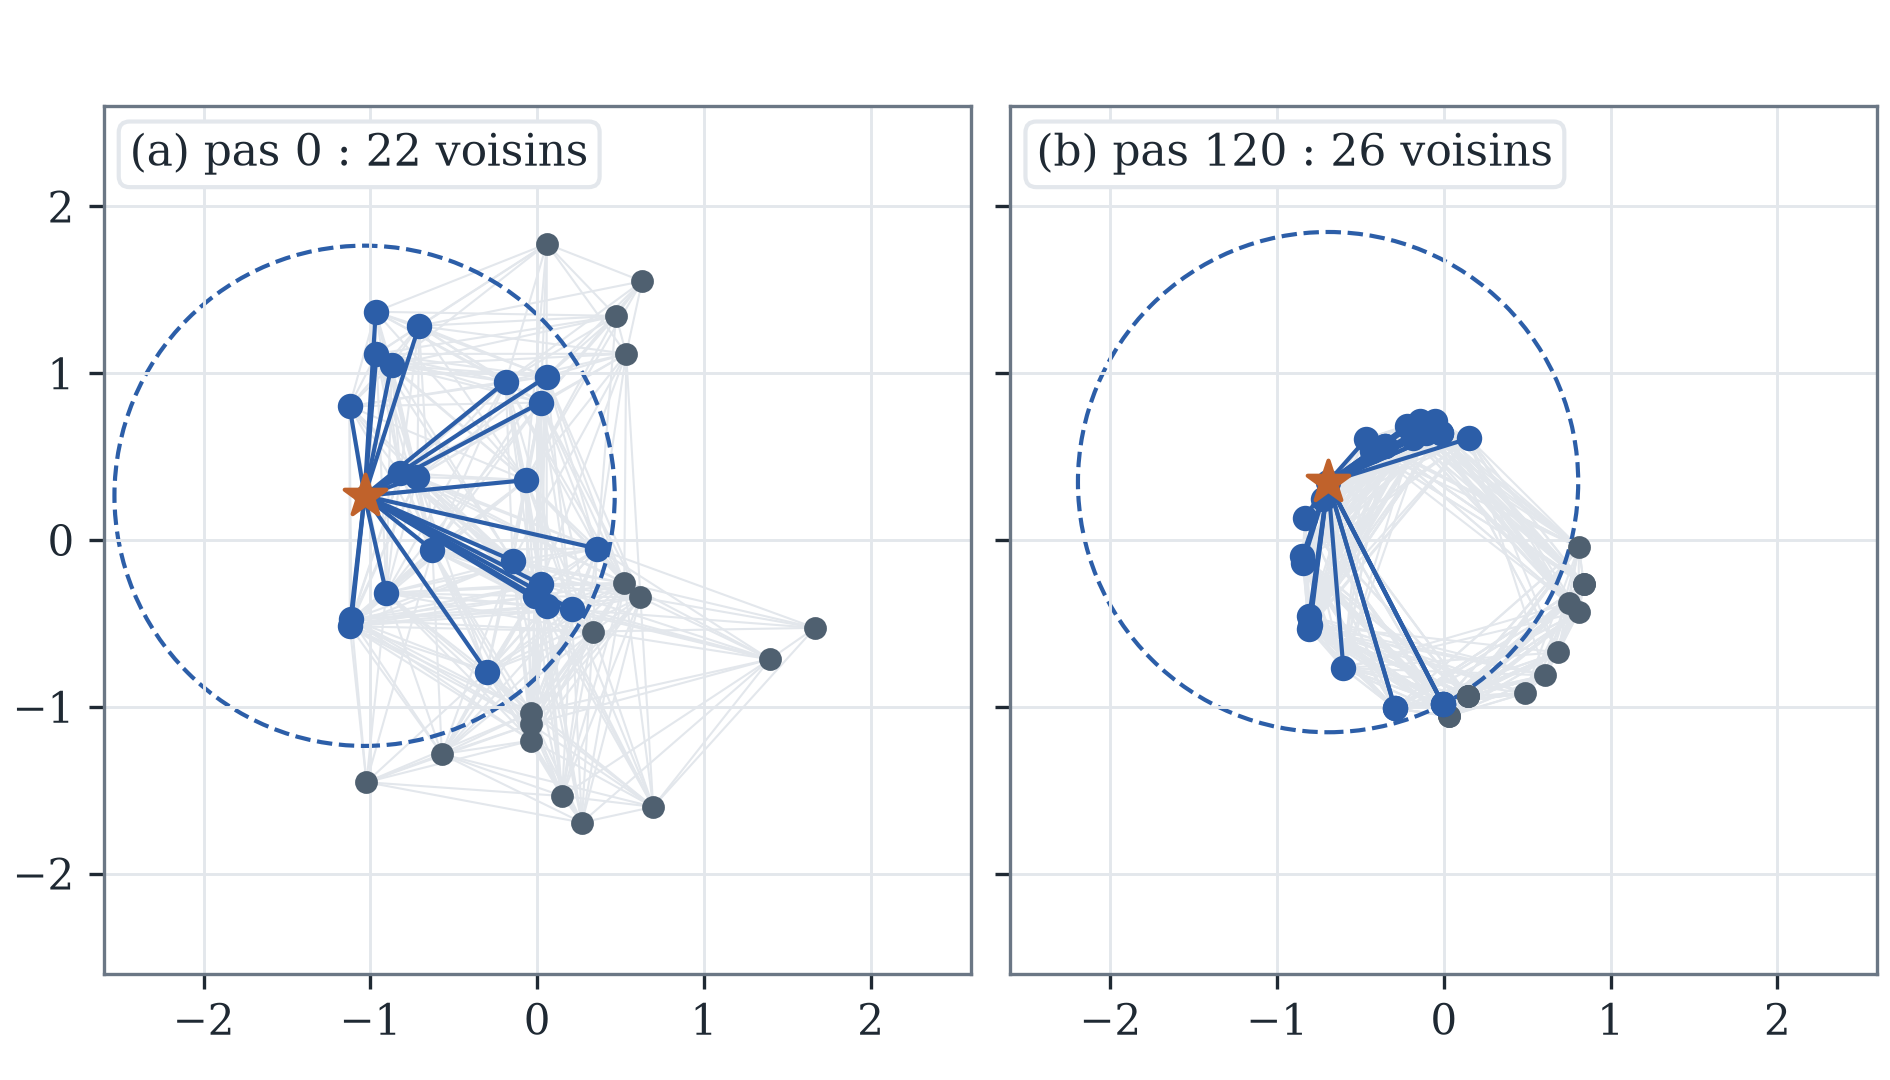
\includegraphics[width=\linewidth,height=.82\textheight,keepaspectratio]{images/real_communication_graph.png}
  \caption[Graphe de communication d'un essaim réel]{Graphe de communication de 40 robots aux pas 0 et 120 (portée 1,5). Le robot étoilé est relié aux robots en bleu, situés dans sa portée (cercle pointillé). Positions lues dans un épisode enregistré de la campagne pilote ; arêtes recalculées à partir de ces positions.}
  \label{fig:communication-graph}
\end{figure}

Deux conséquences touchent directement notre sujet. La première concerne la distance que parcourt l'information. Un lien direct ne transporte que ce que le voisin immédiat transmet. Une information plus lointaine ne parvient à un robot qu'en traversant une chaîne d'arêtes, un tour d'échange par arête. Pendant un pas de simulation, elle ne peut donc pas aller plus loin que le nombre de tours multiplié par la portée.

La seconde concerne la connectivité. Si le graphe se coupe en morceaux, des groupes cessent de recevoir la même information et peuvent partir dans des directions différentes. Les travaux sur le consensus entre agents montrent que l'accord dépend de la connectivité du graphe d'interaction au fil du temps \cite{jadbabaie2003}. Un contrôleur de formation n'hérite d'aucune garantie de ce type. L'avertissement reste valable : il faut suivre la connectivité pendant une expérience.

Enfin, un voisinage est un ensemble non ordonné, de taille variable. Un calcul qui dépendrait de l'ordre dans lequel les voisins sont énumérés produirait des commandes différentes pour une même configuration physique. Cette contrainte, l'invariance par permutation, revient souvent dans la suite.

\section{Réseaux de neurones sur graphes}

Un réseau de neurones sur graphe traite des données organisées en relations, et non en grille ou en liste de taille fixe. Le modèle de Scarselli et al. propage des états entre nœuds reliés jusqu'à atteindre un point fixe, qu'une fonction de sortie transforme en résultat \cite{scarselli2009}. Les architectures actuelles se contentent d'un nombre fini d'étapes, entraînées par rétropropagation \cite{gilmer2017}.

Le déroulement d'une étape se décrit en quatre temps. Chaque nœud encode son état courant et les informations dont il dispose. Chaque arête produit un message à partir des deux nœuds qu'elle relie et de la relation entre eux. Un nœud combine ensuite les messages reçus de ses voisins. Cette combinaison, appelée agrégation, ne doit pas dépendre de l'ordre des voisins, puisque cet ordre n'a pas de sens. Les fonctions invariantes par permutation ont justement été étudiées pour traiter des ensembles non ordonnés \cite{zaheer2017}. Vient enfin une étape de mise à jour, puis un décodeur qui rend la commande attendue. Dans un essaim, les nœuds sont les robots et les messages ne circulent que le long des arêtes du graphe de voisinage. Le chapitre~\ref{chap:methode} détaille les couches du modèle utilisé.

Dans un essaim, tous les robots exécutent la même fonction avec les mêmes poids. Le nombre de paramètres ne dépend donc pas de l'effectif : le même modèle sert pour 20 ou pour 100 robots. Le temps de calcul, lui, augmente avec le nombre de robots. Quand les messages utilisent la position d'un voisin par rapport à soi, et non sa position absolue, la politique ne dépend pas non plus de l'endroit de l'arène où se trouve le groupe.

Il faut en dire les limites. Un réseau à passage de messages reste borné par ce qu'il perçoit : un contrôleur qui ignore une information ne peut pas la reconstituer. Le choix de l'agrégation n'est pas neutre non plus : moyenne, somme et attention n'ont pas le même pouvoir expressif ; les réseaux à attention apprennent un poids propre à chaque voisin \cite{velickovic2018}, ce que la moyenne simple ne fait pas. Enfin, exécuter avec un effectif différent de celui de l'entraînement est possible du point de vue du calcul, mais l'écart réel entre les deux situations doit être mesuré, comme cela a été fait ailleurs sur une formation triangulaire \cite{jiang2023}.

\section{Former une forme, et dire si elle est formée}

Rassembler plusieurs robots dans une même zone ne donne ni un cercle, ni une lettre, ni un symbole. La formation de formes demande que les robots se répartissent sur les différentes parties d'une géométrie visée, tout en évitant de se rapprocher trop les uns des autres. Une règle qui attire tous les robots vers un point commun résout donc un autre problème que celui qui nous occupe.

Représenter la cible se fait de plusieurs manières : une équation analytique, une affectation robot--point, une carte ou un nuage de points. Ces choix ne donnent pas la même information au contrôleur, et plusieurs travaux consacrés à la génération de formes par contrôle décentralisé l'ont montré \cite{hsieh2008,li2019}. Le nuage de points a un avantage pratique : il décrit n'importe quelle forme, même irrégulière, sans expression analytique. Il sert de base aux expériences de ce mémoire.

La qualité d'une formation se juge alors sur deux registres distincts, qu'il serait faux de confondre. D'un côté, savoir si chaque robot actif est proche d'un point de la cible. De l'autre, savoir si chaque partie de la cible est effectivement couverte par un robot. Une politique peut réussir le premier point et échouer au second, en laissant une zone nue : tous les robots se tassent sur un seul arc d'un cercle, par exemple. Une mesure qui additionne ces deux directions, la proximité et la couverture, décrit couramment ce type de tâche. Les collisions, la régularité des espacements entre robots et la connectivité du graphe complètent le tableau. Une forme belle mais instable, ou obtenue au prix de rapprochements dangereux, n'est pas un résultat satisfaisant.

Reste la question du seuil. Une distance moyenne et un taux de succès ne disent pas la même chose, et la convention retenue pour déclarer un épisode réussi change les pourcentages obtenus. Le chapitre~\ref{chap:methode} précise cette convention, parce qu'elle conditionne la lecture de tous les chiffres qui suivent.

\section{Règle écrite et politique apprise}

Deux façons de produire la commande reviennent dans ce mémoire. Écrire la loi de contrôle, c'est fixer soi-même les attractions, les répulsions et parfois les alignements, avec leurs gains et leurs distances d'action. Le résultat reste lisible : quand quelque chose déraille, on remonte à un terme et on le corrige. Le prix est celui de la conception : une forme plus complexe ou une contrainte nouvelle obligent à redériver la loi et à réajuster des paramètres à la main.

Apprendre la loi, c'est déplacer la responsabilité du concepteur. Il ne choisit plus la réaction exacte à chaque configuration, mais ce que les robots perçoivent, la structure du réseau, les objectifs à optimiser et les épisodes sur lesquels entraîner. Les paramètres s'ajustent ensuite. Une observation mal choisie, une perte mal définie ou un entraînement trop court peuvent alors empêcher le modèle d'apprendre, même si le réseau est correctement implémenté.

Il serait simpliste d'opposer une méthode explicable à une méthode opaque. Les deux reposent sur des hypothèses de modélisation. Une règle de flocking suppose que l'attraction, la répulsion et l'alignement suffisent à la mission. Une politique apprise suppose que les exemples vus à l'entraînement couvrent les situations utiles et que la perte favorise bien la formation voulue. Le mémoire ne cherche pas à décider quelle famille est la meilleure. Il cherche à savoir dans quelles conditions une règle apprise, exécutée localement, peut remplacer une règle écrite à la main.

\section{Conclusion partielle}

Un essaim se pilote par décisions locales et échanges limités, et cette décentralisation porte sur l'exécution, pas forcément sur l'apprentissage. Le voisinage, défini par une portée de communication, forme un graphe reconstruit à chaque pas, de sorte qu'une information ne circule qu'aussi loin que le permettent les tours d'échange et la connectivité. Un réseau de neurones sur graphes y applique une même fonction à tous les nœuds, à condition que l'agrégation reste invariante par permutation. Une formation de formes, enfin, se juge en deux directions, la proximité des robots à la cible et la couverture de la cible par les robots, et non par un regroupement. Le chapitre suivant confronte ces notions aux travaux existants, méthodes traditionnelles puis approches apprises, et examine trois études dont la comparabilité avec notre protocole n'allait pas de soi.
